\documentclass{beamer}
\usepackage{graphics}
%\usepackage[latin1]{inputenc}
\usetheme{CambridgeUS}
\title[Research articles]{Inverse methods: Hybrid Data Assimilation}
\author{Ksenia Kozhanova, Maxime Mazouth--Laurol, Michi Rakotonarivo}
\institute{Grenoble INP, MSIAM 2}
\date{January, 2018}
\begin{document}

\begin{frame}
\titlepage
\end{frame}

\begin{frame}
\frametitle{Variational Methods}
\pause
\begin{definition}
	\textbf{Data assimilation} (or data analysis) is the process by which observations of the actual system are incorporated into the model state of a numerical model of that system
\end{definition}

\pause
\begin{itemize}
	\item $\mathbf{w}$ is a state vector, $M$ is a model, $\mathbf {M} = \mathbf {M}(t_{i}, t_{i-1})$ is a linear operator related to $\delta \mathbf {w(t_{i-1})}$ and $M(t_{i},t_{i-1})$ is a non-linear model operator related to $\mathbf {w(t_{i-1})}$
	\item $ \mathbf{w} = \mathbf {w^{b}}+\delta \mathbf {w}$
	\item $\mathbf {w}(t_{i})=M(t_{i},t_{i-1})[\mathbf {w}(t_{i-1})]$
\end{itemize}
\end{frame}


\begin{frame}
	\frametitle{4DVAR}
	
	\pause
	\begin{itemize}
		\item $\mathbf {w}(t_{i}) \approx M(t_{i},t_{i-1})[\mathbf {w}^{b}(t_{i-1})] + \mathbf {M}(t_{i},t_{i-1})\delta \mathbf {w}(t_{i-1})$
		\item $\delta \mathbf {w}(t_{i}) = \mathbf {M}(t_{i},t_{i-1})\delta \mathbf {w}(t_{i-1})$
		\item $\mathbf {w}(t_{i})=M(t_{i},t_{i-1})[\mathbf {w}(t_{i-1})]$
		\item $J(\delta \mathbf {w}) = \frac{1}{2} \delta \mathbf {w}^{T} \mathbf {B}^{-1} \delta \mathbf {w} + \frac{1}{2} \sum_{i=0}^{n}(\mathbf {G}_{i} \delta \mathbf {w} - \mathbf {d}_{i})^{T}\mathbf {R}_{i}^{-1}(\mathbf {G}_{i} \delta \mathbf {w} - \mathbf {d}_{i})$
		where $\mathbf {B}$ and $\mathbf {R}_{i}$ are matrices with covariance estimates of background and observation error, $G_{i} = H_{i}M(t_{i},t_{0})$ being a generalized observation operator, $\mathbf {G}_{i} = \mathbf {H}_{i}\mathbf {M}(t_{i},t_{0})$ being a linear observation operator
	\end{itemize}
\end{frame}


\begin{frame}
	\frametitle{4DVAR vs 3DVAR}
	\begin{itemize}
		\item The difference comes from the choice of $\mathbf{M}$ to obtain linearised observation operator $\mathbf {G}_{i}$
		\item 3DVAR: $\mathbf {M} = \mathbf {I}$, where $\mathbf {I}$
		\item 4DVAR: $\mathbf {M} \approx (\partial M/\partial \mathbf {w})|_{w-w^{b}}$
	\end{itemize}
\end{frame}


\begin{frame}
	\frametitle{Kalman theory}
	\begin{itemize}
		\item Analysis equation $\psi ^{a} = \psi ^{f} + \textbf{P} ^{f}\textbf{H} ^{T}(\textbf{HP} ^{f}\textbf{H} ^{T}+\textbf{R}) ^{-1}(\textbf{d-H}\psi) ^{f}$
		\item $\textbf{P}^{a} = \textbf{P}^{f} - \textbf{P}^{f}\textbf{H}^{T}(\textbf{HP}^{f}\textbf{H}^{T}+\textbf{R})^{-1}\textbf{HP}^{f} $ 
		\item where  $\textbf{P}^{.}$ is the covariance for the model forecast/analysis,  $\textbf{R}$ is the covariance for the model measurements, $\textbf{H}$ is the measurement operator
		
	    \item Error covariance $\textbf{P}_{k+1}=\textbf{F}\textbf{P}_{k}\textbf{F}^{T}+\textbf{Q}$
	    \begin{itemize}
	    	\item Traditional Kalman filter: linear model $\psi_{k+1}=\textbf{F}\psi{k}$
	    	\item Extended Kalman filter: non-linear model
	    	$\psi_{k+1}=\textbf{f}(\psi_{k})$
	    	
	    \end{itemize}
	\end{itemize}
\end{frame}


\begin{frame}
	\frametitle{Ensemble Kalman filter}
	
	\begin{definition}
		\textbf{Ensemble forecasting} is the process where multiple, individual numerical forecasts
		are generated from different sets of initial conditions
		and/or different numerical model configurations (Leith 1974)
	\end{definition}
	\begin{itemize}
		
		\item error covariance $\textbf{P}_{e}^{a} = \overline {(\psi^{a} - \overline{\psi^{a}})(\psi^{a} - \overline{\psi^{a}})^{T}} =  (\textbf{I}-\textbf{K}_{e}\textbf{H})\textbf{P}_{e}^{f}$, 
		where $\textbf{K}_{e}$ is Kalman gain
		\item if we have infinite number of ensembles, we have traditional Kalman filter

	\end{itemize}
\end{frame}

\begin{frame}
	\frametitle{Hybrid methods}

	\begin{itemize}
		
		\item En3DVAR covariance matrix: $\textbf{P}^{b}_{i} = (n-2)^{-1} \sum_{j=1, j \ne i}^{n}(\textbf{x}_{j}^{b} - \overline{\textbf{x}}_{i}^{b})(\textbf{x}_{j}^{b} - \overline{\textbf{x}}_{i}^{b})^{T}$
		
		\item En4DVAR
		\begin{itemize}
			\item 4DVAR cost function $J(\textbf{w}) = \frac{1}{2} \textbf{w}^{T}\textbf{w} + \frac{1}{2}(\textbf{H}\textbf{X}'_{b}\textbf{w}+\textbf{d})^{T}\textbf{O}^{-1}(\textbf{H}\textbf{X}'_{b}\textbf{w}+\textbf{d})$
			\item En4DVAR cost function $J(\textbf{w}) = \frac{1}{2} \textbf{w}^{T}\textbf{w} + \frac{1}{2}\sum_{i=0}^{I}(\textbf{HM}\textbf{X}'_{b}\textbf{w} + \textbf{d}_{i})^{T}\textbf{O}^{-1}(\textbf{HMX}'_{b}\textbf{w}+\textbf{d}_{i})$
			\item background error in observation space:
			$\textbf{HMX}'_{b} \approx \frac{1}{\sqrt{N-1}}(HM\textbf{x}_{b1}-HM\overline{\textbf{x}_{b}}, HM\textbf{x}_{b2}-HM\overline{\textbf{x}_{b}},.....,HM\textbf{x}_{bN}-HM\overline{\textbf{x}_{b}} )$
			\item recomputed gradient of the cost function $\nabla _{w}J = \textbf{w} + \sum_{i=0}^{I}(\textbf{HMX}_{b}')^{T}\textbf{O}^{-1}(\textbf{HMX}_{b}'\textbf{w}+\textbf{d}_{i})$
		\end{itemize}
		
	\end{itemize}
\end{frame}

\section{Motivation}
\subsection{Initialization}
\begin{frame}
	\frametitle{Advantages of En4DVAR}
	
	\begin{itemize}
		
		\item combination of the unique benefits of each approach 
		\item relaxation of the requirement to have tangent linear model or adjoint model
		\item similar results with smaller computational cost
		\item appropriate data assimilation method due to the non-sequential nature
		
	\end{itemize}
\end{frame}


\section{Iterative Ensemble Kalman Smoother}
\begin{frame}
\frametitle{Statements}
The Iterative Ensemble Kalman Smoother(IEnKS) follows the same scheme than standard Ensemble Kalman Filter :
\begin{itemize}
\item Ensemble forecast
\item Analysis
\item Posterior ensemble generation
\end{itemize}

But there are differences :
\begin{itemize}
\item  Analysis is variational
\item  Gradient of the cost function approximated using the ensemble
\end{itemize}
\end{frame}

\begin{frame}
\frametitle{Algorithm}
\begin{itemize}
\item $L$ : size of the Data Assimilation Window(DAW)
\item $S$ : number of forecast steps
\end{itemize}
\begin{center}
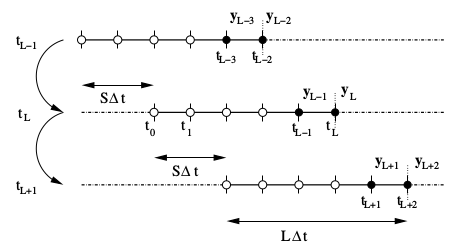
\includegraphics[scale=0.5]{../Image/IEnKS_chaining.png} 
\end{center}
Here, $L=5$ and $S=2$.
\end{frame}


\begin{frame}
\frametitle{Data assimilation monitoring}
The defined cost function :
$$\tilde{J}(w) = \frac{1}{2}(N-1)\textbf{w}^{T}\textbf{w} + \frac{1}{2}\sum_{k=1}^{L}\beta_{k}\delta_{k}^{T}(\textbf{w})\textbf{R}_{k}^{-1}\delta_{k}(\textbf{w})$$

\begin{itemize}
\item $\{\beta_k\}_{k \in [\![1,L]\!]}$ : observation weights
\item $L$ and $S$ : Overlap between consecutive DAWs.
\end{itemize}
\end{frame}

\begin{frame}
\frametitle{Numerical experiment}
\textbf{Problem statement} \\
Twin experiments together with the following Lorenz-95 model : \\
\begin{equation*}
\frac{dx_m}{dt} = (x_{m+1}-x_{m-2})x_{m-1} - x_m + F
\end{equation*}
with $x_m, m \in [\![1,M]\!]$ a variable and F the forcing parameter. \\

\textbf{Measurement metric}
$$\operatorname{RMSE}= \sqrt{\frac{\sum_{t=1}^M (x_{m}^{a} - x_{m}^{t})^2}{M}}.$$
\end{frame}
\begin{frame}
\frametitle{Overview of the results}
\framesubtitle{Parameter F known}
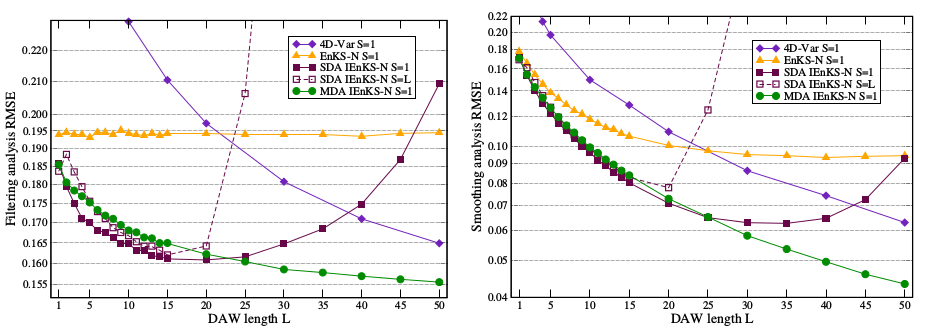
\includegraphics[width=\paperwidth,height=\paperheight]{../Image/IEnKS_weak.png}

\end{frame}

\begin{frame}
\frametitle{Augmented state principle}
\begin{itemize}
\item state vector $\textbf{x} \in \mathbb{R}^M$
\item vector of parameters $\textbf{p} \in \mathbb{R}^P$
\end{itemize}

Then, the augmented state vector is z = (x,p) 
\begin{center}
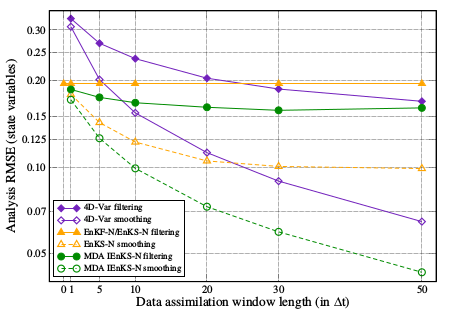
\includegraphics[scale=0.5]{../Image/IEnKS_forcing.png}
\end{center}
\end{frame}

\end{document}